\documentclass[a4paper]{article}

% Options possibles : 10pt, 11pt, 12pt (taille de la fonte)
%                     oneside, twoside (recto simple, recto-verso)
%                     draft, final (stade de développement)

\usepackage[utf8]{inputenc}   % LaTeX, comprends les accents !
\usepackage[T1]{fontenc}      % Police contenant les caractères français
\usepackage[francais]{babel}  


\usepackage[a4paper,left=2cm,right=2cm]{geometry}% Format de la page, réduction des marges
\usepackage{graphicx}  % pour inclure des images

\usepackage{algorithm}
\usepackage{algpseudocode} % algorithme
% \usepackage{algcompatible}
% \usepackage{algorithm2e}

%\pagestyle{headings}        % Pour mettre des entêtes avec les titres
                              % des sections en haut de page

\title{  Qui est-ce ?\\         % Les paramètres du titre : titre, auteur, date
Projet de programmation}          
\author{Groupe \emph{Z}\\
  \emph{Frédéric,Laurent,Tony et Romain}\\
  \emph{https://gitlab.etu.umontpellier.fr/e20180001091/qui-est-ce}\\
  L2 informatique\\
  Faculté des Sciences\\
Université de Montpellier.}
\date{\today}             

\renewcommand*\contentsname{Sommaire}

\begin{document}

\maketitle
\begin{center}
    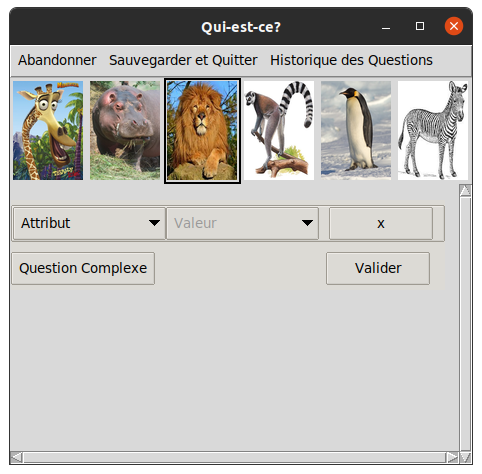
\includegraphics[scale=0.7]{./fenetreJeu.png}
\end{center}
\clearpage

\newpage
\tableofcontents
\clearpage


\begin{abstract}     % Résumé du travail
  \emph{Le but est de créer un Qui-est-ce? Pour cela nous avons d'abord créer le jeu, puis un générateur de plateau compatible. Tout cela utilsable par interface homme-machine graphique.}
\end{abstract}

\section{Technologies utilisées  et organisation}
\subsection{Choix du langage}
\paragraph*{Nous avons choisi Python,} il s'agit d'un langage populaire avec une communauté active et nous n'avons pas eu de mal à trouver de l'aide ou des exemples.
De plus, le langage est simple et sa syntaxe courte nous a permis de réaliser notre projet relativement rapidement.
Puisque Python est Orienté Objet, nous avons réussi a mettre une structure du code acceptable.
La POO nous a permis de diviser les tâches à réaliser et les répartir facilement.
Finalement le code sera portable (Write Once, Run Anywhere) et cela nous a été précieux étant donnée que nous n'utilions pas le même environnement de travail.
\paragraph*{Bibliothèques, framework, ... utilisés:}
\begin{itemize}
\item Tkinter est installé par défaut sinon éxécuter (python3 -m tkinter) depuis la ligne de commande.Cela ouvrira une fenêtre de démonstration d'une interface Tk simple en indiquant que tkinter est correctement installé sur votre système et indiquant également quelle version de Tcl/Tk est installée\\
\item Pillow pour lire des images au format jpg/png
\end{itemize}

\subsection{Organisation du travail}
\paragraph{Répartition du travail au sein du groupe}

  - 4 personnes au sein du groupe: Romain, Frédéric ,Laurent et Tony
  \subparagraph{}
  Jeu de base:
  \begin{itemize}
  \item Romain : fonctions du jeu de base + interface graphique
  \item Frédéric : interface graphique
  \item Laurent + Tony : fonctions du jeu de base
  \end{itemize}

  \subparagraph{Générateur:}

  \begin{itemize}
    \item Frédéric : fonctions du générateur
    \item Tony : fonctions du générateur
    \item Laurent : Interface du générateur + fonctions du générateur 
    \item Romain : Interface du générateur
  \end{itemize}
   
   
  \paragraph{Rythme de travail:} 3h/semaine en td + heures suplémentaires à la BU \\
 \subparagraph{Mode de fonctionnement:}
 \begin{itemize}
 \item Premier partie ->   modele UML + organisation des taches à se répartir\\
 \item Deuxième partie ->  Exécution de l'organisation  
 \end{itemize}

 \clearpage
 \section{Étape 1 : permettre à l'utilisateur de jouer}

 \subsection*{Fonctionnalités de l'application : interactions possibles de l'utilisateur}
 
 \paragraph*{}
 Le jeu (de base)
 
 Après avoir lancé le terminal, nous entrons notre nom, choissisons le plateau, puis mode facile ou difficile.
 
 Une fois en jeu, nous pouvons coché des portrait (clic gauche) et accuser un personnage (clic droit)
 En bas de la fenêtre, des bouttons nous permettent de créer notre question, de la poser puis voir la réponse.
 Un haut, un petit menu vous permettra de sauvegarder la partie en cours, voir votre historique de question et abbandoner.
 
 \paragraph*{}
 Le générateur
 
 Le joueur doit lancé le générateur par le terminal en choisisant en paramètre le thème.
 
 En ce qui concerne les métadonnées (taille de la grille, des images), il est possible de les modifier si les valeurs par défaut ne conviennent pas.
 
 Ensuite, l'utilisateur doit définir des attributs puis y ajouter des valeurs afin de les utiliser par la suite.
 
 Par ailleurs, les attributs avec leurs valeurs peuvent être donner à des personnages.
 
 Il n'y a pas d'autré pré-établi si ce n'est que il vous faut au moins un attribut avec au moins 1 valeur pour pouvoir la donner à un personnage. 
 
 Nous avons la possibilité d'ajouter des attributs, d'ajouter des valeurs à ces attributs, modifier et supprimer. Ces Fonctionnalités ont des répercussions sur les personnage qui les portent.
 
 
 \subsection*{Format du fichier JSON, contraintes éventuelles}
 "metadonnees" Cette clé renvoie vers des données essentiels pour le bon fonctionnement de l'interface graphique.\\
 "images" contient le chemin vers le dossier contenant les images depuis la racine du projet \\
 "ligne" et "colonne" forment la taille de la grille\\
 "largeurImage" et "hauteurImage" correspond à la définition de chaque portrait à l'écran (!= la définition réel des images dans le dossier)\\
 "espacementPhoto" est l'espacement entre les portrait sur l'interface graphique\\
 "possibilites"\\
 Chaque clé correspond à la représentation d'un personnage.
 Chaque personnage doit avoir les clés "fichier" et "nom".
 Le reste des clés du personnages correspond aux noms de ces attributs.
 Les clés des personnages sont associés à des liste pour permettre la multiplicité des valeurs.
 Les personnages ont le même nombre d'attribut.
 
 \begin{figure}
   \caption{Squelette type de nos fichier JSON}
   \centering
   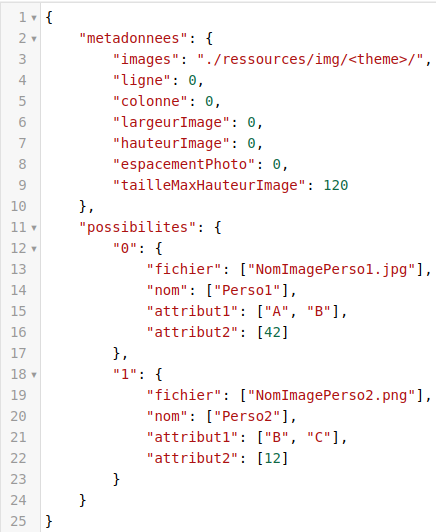
\includegraphics[scale=0.15]{./squeletteJSON.png}
 \end{figure}
 
 \clearpage
 \subsection*{Description des structures de données, classes, variables}
 \paragraph*{La classe Jeu} ne contient pas de logique. Elle sert simplement à réunir les autres objets dans un unique objet, facilité la création des objets et contient quelques méthodes "utiles".
 La méthode calculeMapAttributsDomaine() renvoie les attributs et leurs valeurs sous forme de dictionnaire pour l'interface
 Nous considérons que poser une question sur le nom d'un personnage et sur ses attributs sont philosophiquement différentes, par conséquent il d'un côté accuser() pour identifier ou pas notre personnage mystère et evaluer() pour poser des questions.
 
 \begin{figure}
   \caption{Diagramme de classe du jeu}
   \centering
   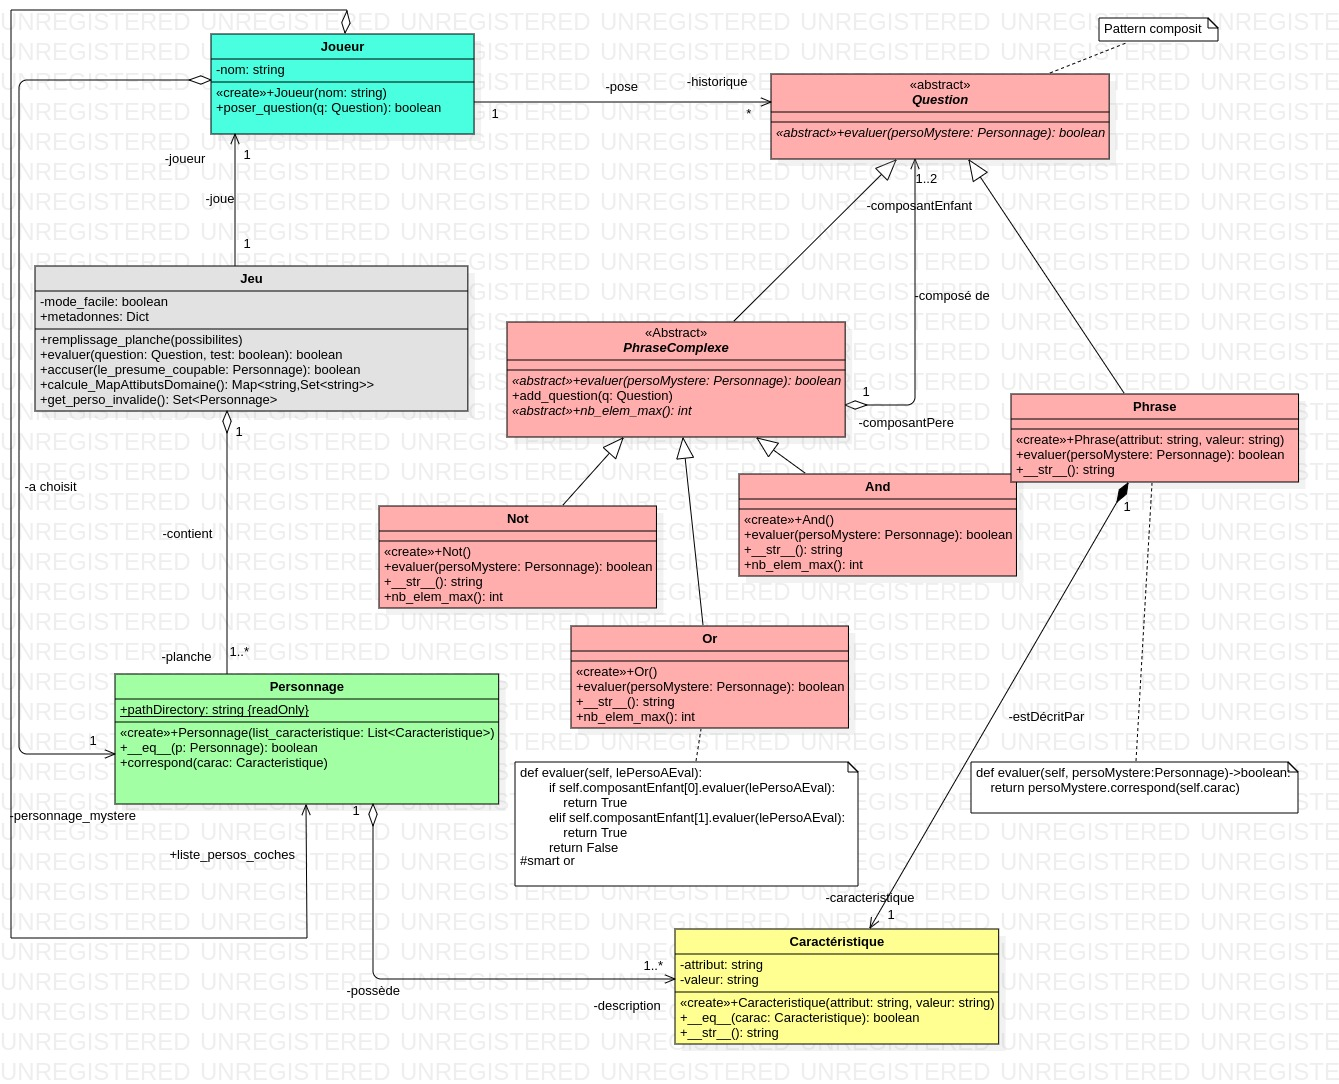
\includegraphics[scale=0.35]{./JeuClassDiagram.jpg}
 \end{figure}
 
 \clearpage
 \subsection*{Description de la forme des requêtes traitées et un traitement.}
 \begin{figure}
   \caption{Diagramme objet représentant une question}
   \centering
   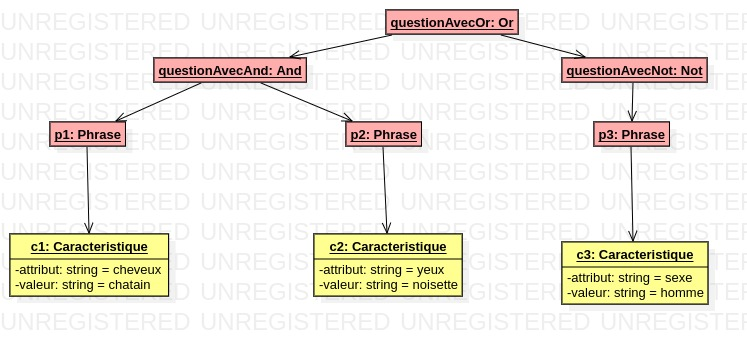
\includegraphics[scale=0.4]{./requetesObject.jpg}
 \end{figure}
 \paragraph*{}
 Nous avons choisit d'utiliser un pattern composite pour représenter les questions.
 En effet, la situation si prete bien. Puisque dans notre Qui-est ce?, nous voulons qu'un utilisateur puisse intéroger sur plusieurs choses à la fois tout en représetant sufisament précisement la complexité d'une question.
 Nous voullons qu'une question puisse en contenir d'autre et être relié par un connecteur logique donné.
 En cela, le composit pattern remplis notre besoin car une question est un arbre dont les différents nœuds sont des connecteurs logiques, et les vrais questions sont les feuilles de cette arbre. Et un sous arbre serait également une question valide.
 
 
 \subsection*{Description du traitement effectué lors d'une requête.}
 \begin{figure}
   \caption{Diagramme de séquence, le joueur pose une question}
   \centering
   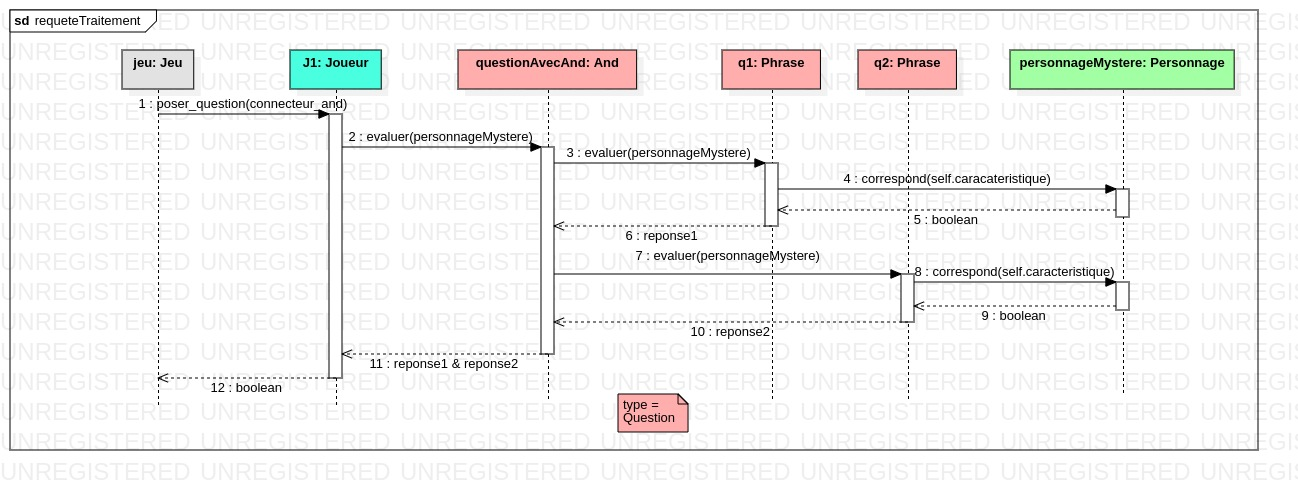
\includegraphics[scale=0.38]{./requeteTraitement.jpg}
 \end{figure}
 
 \paragraph*{}Lorsque que le joueur pose une question (1), l'objet J1 de type Joueur va passé le personnage mystère pour que la question qu'il veut posé puisse être évaluer.
 La question questionAvecAnd va s'évaluer (2) récursivement avec ces enfants (3,7) jusqu'à qu'elle tombe sur une feuille. Les phrases au bout de l'arbre vérifie si ils correspond au personnage passé en argument (4,8).
 \clearpage

 \section{Étape 2 : aider  à la saisie  des personnages}
 \subsection{Description du problème: format des données et du résultat}
 Premièrement, au début de la programmation, nous avions eu deux choix de concept pour l'attribution des caractéristiques aux personnages depuis l'interface:
 \begin{itemize}
 \item {Saisir manuellement (au clavier) chaque attributs, valeurs de chaque personnages}
 \item {Créer les attributs et les valeurs associées, les stockers, puis les attribuer aux personnages en les sélectionnant} 
 \end{itemize}
 Comme les deux concepts possédaient des avantages et des inconvénients, nous avions décidé d'établir la liste de celles-ci afin de déterminer la meilleure des deux.
 \begin{itemize}
 \item {Pour la saisie manuelle :}
 \end{itemize}
 
 L'avantage :\\  
   - Développement d'apparence plus simple (peu de fonction à implémenter)\\
 
 Les inconvénients :\\
   - Malgré la possibilité de vérifier les occurrences par comparaison orthographique, un "non" != "Non" != "Nope" donc possibilité d'occurence\\
   - Dans le cas d'une envie de modifier ou de supprimer un attribut ou une valeur, il faudrait apporter la modification manuellement pour chaque personnage\\
   - Complexifie les méthodes de vérification de la validité des données\\
   - Saisie inconfortable des caractéristiques
 \begin{itemize}
 \item {Pour la saisie des caractéristiques et leur attribution aux personnage par simple selection :}
 \end{itemize}
 
 Les avantages :\\
 - Vérification de la validité des données plus simple (unicité des caractéristiques des personnages)\\
 - Modification et de suppression des caractéristiques plus confortable et rapide\\
 
 (!) Possibilité d'attribuer automatiquement les attributs déjà créés aux personnages\\
 
 (!) Lors de la modification ou de la suppression d'un attribut ou d'une valeur, chaque personnage ayant cet attribut ou cette valeur recevra une modification automatique au niveau de sa liste de caractéristique\\
             
 Les inconvénients :\\
 - Malgré la possibilité de vérifier les occurrences par comparaison orthographique, un "non" != "Non" != "Nope" donc possibilité d'occurence\\
 - Complexification du développement\\
 
 (!) Création d'une class de type fenêtre pour la création et la modification des caractéristiques\\
 
 (!) Création d'une class de type fenêtre pour l'attribution des valeurs aux attributs des personnages\\              
 
 Après reflexion, nous avions alors opté pour le deuxième concept en raison de fait que malgré la complexité du codage, le générateur serait beaucoup plus agréable à utiliser et de meilleur qualité.\\
 
 Deuxièmement, après s'être mis d'accord sur la manière de saisie des données, il n'y avait plus qu'à réfléchir 
 sur la manière de récupérer les données de chaque personnage.\\
 Comme les paramètres de configuration de l'interface et le nom du plateau du qui-es-ce sont contenus directement dans les attributs du générateur, il à été facile de les récolter. 
 Cependant, les personnages sont des objets de class et que leurs données ont été placées dans leurs attributs, nous avions alors implementé une fonction parcourant les personnages un à un avec leurs attributs. Au fur et à mesure, la fonction 
 récolter alors leurs données sous la forme d'une String, et lorsque tout les personnages ont été parcouru,
 les données des personnages et de la configuration de l'interface du qui-es-ce sont écrites dans un fichier Json généré automatiquement et dont le nom est donnée en fonction du nom du dossier contenant les images des différents personnages.
 
 \subsection{Scénario des interactions avec l'utilisateur}
 \begin{enumerate}
 \item L'utilisateur exécute le programme : 
 \begin{itemize}
     \item (sans sauvegarde) il saisit la commande pour exécuter le programme suivit du chemin vers les images
     \item (avec sauvegarde) il saisit la commande pour exécuter le programme suivit de l'option -save
 \end{itemize}
 \item Le main initialise l'interface
 \item L'utilisateur configure l'interface avec les entry :
 \begin{itemize}
     \item Il saisie des dimensions du plateau 
     \item Il saisie de la taille des images représentant les personnages
     \item Il saisie l'espacement entre les images
 \end{itemize}
 
 (!) Le générateur affiche d'un messages d'erreur si les dimensions de la grille ne conviennent pas, si la taille d'image est trop grande ou si l'espacement entre les images est trop grand
     
 \item L'utilisateur crée les caractéristiques avec le bouton "configuration Attributs"
 \item Le générateur affiche une nouvelle fenêtre permettant à l'utilisateur de créer les caractéristiques 
 \begin{itemize}
     \item l'utilisateur créé / modifie ou supprime des attributs et les valeurs correspondant
 \end{itemize}
 
 (!) affichage d'une erreur s'il y a la création d'un attribut déjà existant\\
 
 (!) affichage d'une erreur si la modification du nom d'un attribut correspond à un autre\\
 
 (!) affiche une demande de confirmation si vous effectué une modification et affichage d'un avertissement si vous voulez supprimer un attribut ou une valeur
 \item L'utilisateur affiche l'aperçu du plateau en cliquant avec le bouton "Aperçu"
 \item L'utilisateur caractérise les personnages du plateau :
 \begin{itemize}
     \item Clique sur l'image d'un des personnage sur l'aperçu du plateau 
     \item Le générateur affiche les attributs existant
     \item Selection des valeurs correspondant aux attributs du personnage et valide la selection 
 \end{itemize}
 
 (!) affichage d'une erreur si le dictionnaire description du personnage n'est pas unique
 
 \begin{itemize}
     \item Répétition du même processus pour tout les personnages du plateau
 \end{itemize}
 
 \item Le générateur verifi la validité du plateau :
 \begin{itemize}
     \item Il vérifie si toutes les caractéristiques de chaque personnage ont été attribuées d'une ou de plusieurs valeurs 
 \end{itemize}
 
 (!) affichage d'un message d'erreur si des personnages ont été mal caractérisés (application d'un filtre rouge sur l'image des personnage mais caractérisés / application d'un filtre vert dans le cas contraire)
 
   \begin{itemize}
     \item Si tout a été correctement fait, le générateur affiche un message indiquant la génération du fichier .json
 \end{itemize}
 \end{enumerate}
 
 \clearpage
 \section{Étape 3: Jouer sur deux ordinateur et contre l'ordinateur}

 \subsection{Bot}
 \paragraph{}
 Cette extention vise à créer une petite IA qui pose des question en même temps que le joueur joue pour tenter de trouver son personnage mystère avant l'adversaire\\
 Notre stratégie sera de poser la question qui concerne le plus de personnage suspect. On espère que potentielement, la question posé inocente un grand nombre de personnage.
 \begin{algorithm}
  \caption{TrouverLePersonnageMystère}
  \begin{algorithmic}[1]
    \State $lesSuspects \gets jeu.planche$ \Comment{tout les personnages sont suspects au départ}
    \While{$taille(lesSuspects) \neq 1$}
    \State $carac \gets getCaracteristiquePartagerParlePlusDePersonnageDans(lesSuspects)$
    \State $reponse \gets poserQuestionAProposDe(carac)$
    \State $eliminerSuspects(lesSuspects, carac, reponse)$
    \EndWhile
    \State return $lesSuspects[0]$
  \end{algorithmic}
\end{algorithm}


 \subsection{Réseau}

 \paragraph*{}
 \subparagraph*{}
 La partie réseau a posé beaucoup de problème et demandé un certain temps.
 Cette extention nous permet de jouer à Qui-est ce sur 2 ordinateurs différents sur un même réseau.
 Nous avons opté pour une structure hôte/client.
 L'hôte choisit le plateau de jeu en option lançant par ligne de commande le jeu. 

 \subparagraph*{Le protocole de l'hote}
 \begin{enumerate}
  \item J'envoie le nom du plateau
  \item *discussion*
  \item kill le processus si envoie/reçoit "Goodbye"
  \item son parent ferme la connexion
 \end{enumerate}
 \subparagraph*{Le protocole de l'invité}
 \begin{enumerate}
  \item Je reçoit le nom du plateau
  \item *discussion*
  \item kill le processus si envoie/reçoit "Goodbye"
  \item son parent ferme la connexion
 \end{enumerate}
 \subparagraph*{}
 Chaque joueur sur son ordinateur a 2 processus. Le processus avec l'interface et son processus enfant qui écoute en permanence le socket.
Le chat n'est pas bloquant. Vous pouvez envoyer autant de message à la suite que vous voulez et l'autre joueur vous répond quand il veut. Les messages ne sont \textbf{absolument pas} formaté ni codifié. Nous pouvons demander n'importe quoi, et recevoir n'importe quoi. Ceci a été fait de cette façon pour soucis de simplicité et de temps.

 \clearpage
 \section{Bilan et Conclusions}

 \paragraph{Nous avons rencontré quelques problèmes.}
 En effet, git a été un gros problème pour nous. Partager notre travail entre nous a couté beaucoup de temps. De plus, lors de chaque rendu, nous avons fait des modifications jusqu'à la dernière minute. Ce qui en a causé quelques problèmes et une grande quantité de stress.
 Ensuite, les différents système d'exploitation utilisés au sein de notre groupe ont causé des conflits que nous n'avons pas toujours réussi à résoudre.
 De la même façon, les différentes versions de Python ont elles aussi étaient problématique.
 % \end{itemize}
 
 \paragraph{Mais, nous avons terminé le projet}
 La cohésion du groupe et le travail régulier nous a permis d'avancer rapidement lors de la réalisation du projet.
 Le jeu ainsi que le générateur fonctionne.
 
 

\end{document}
